\documentclass[sigconf]{acmart}
\usepackage{glossaries}
\usepackage{float}
\usepackage{easy-todo} % Todo notes e.g. \todo{note} Creates a note that shows the text “note”.
\usepackage{minted}
\usepackage{titlesec}
\usepackage{enumitem}
\makenoidxglossaries

\settopmatter{printacmref=false}
\setcopyright{none}
\renewcommand\footnotetextcopyrightpermission[1]{}

\setcopyright{none}
\acmConference[SM2-PRO]{}{Group/Individual}{Hand-in}
\makeatletter
\renewcommand\@formatdoi[1]{\ignorespaces}
\newcommand{\code}[1]{\texttt{#1}}
\newcommand{\refappendix}[1]{\hyperref[#1]{Appendix~\ref*{#1}}}
\titleformat*{\paragraph}{\itshape\bfseries}
\titleformat*{\subsubsection}{\bfseries}
\makeatother

\newacronym{msd}{SM2-MSD}{Model-Driven Software Development}
\newacronym{sm-iot}{SM2-IoT}{Software Engineering of Internet of Things}
\newacronym{ssav}{SM-SSAV}{Software System Analysis and Verification}
\newacronym{dsl}{DSL}{Domain-Specific Language}
\newacronym{wan}{WAN}{Wide Area Network}
\newacronym{pi}{RPI4}{Raspberry Pi 4b}
\newacronym{nat}{NAT}{Network Address Translation}
\newacronym{wlan}{WLAN}{Wireless Local Area Network}
\newacronym{iiot}{IIoT}{Industrial Internet of Things}
\newacronym{mqtt}{MQTT}{Message Queue Telemetry Transport}
\newacronym{ap}{AP}{Access Point}
\newacronym{iot}{IoT}{Internet of Things}

\pagestyle{plain}
\settopmatter{printfolios=true}
\begin{document}

\title{Reconfigurable Storing, Scanning and Moving Installation}
\subtitle{Group 01}

\author{Frederik Alexander Hounsvad}
\affiliation{%
  \institution{University of Southern Denmark}
   \city{Odense}
   \country{Denmark}
}
\email{frhou18@student.sdu.dk}

\author{Nikolai Emil Damm}
\affiliation{%
  \institution{University of Southern Denmark}
   \city{Odense}
   \country{Denmark}
}
\email{nidam16@student.sdu.dk}

\author{Peter Andreas Brændgaard}
\affiliation{%
  \institution{University of Southern Denmark}
   \city{Odense}
   \country{Denmark}
}
\email{pebra18@student.sdu.dk}

\author{Oliver Lind Nordestgaard}
\affiliation{%
  \institution{University of Southern Denmark}
   \city{Odense}
   \country{Denmark}
}
\email{olno18@student.sdu.dk}

\author{Troels Zink Kristensen}
\affiliation{%
  \institution{University of Southern Denmark}
   \city{Odense}
   \country{Denmark}
}
\email{tkris17@student.sdu.dk}

\maketitle

%Group report

\section{Group report}
\subsection*{Extended Summary}

The extended features to the system touch upon the following aspects of \acrshort{sm-iot}, \acrshort{msd}, \acrshort{ssav}:

\begin{itemize}[leftmargin=*]
    \item \acrshort{sm-iot}: Health Monitoring of services, connectivity, safe deployment of services, auto-deployment of services.
    \item \acrshort{msd}: Xtext, Xtend, Extended Grammar, Code-generation to multiple targets, left-factoring.  
    \item \acrshort{ssav}: UPPAAL Queries with support for $A[]$, $A<>$, $E[]$, $E<>$, leads to ($\rightarrow$) negation ($!$), conjunction (and/or), and imply.
\end{itemize}

\subsection*{Additional materials}

A video demonstrating the new features is available as an attachment to the project handin. The video demonstrates the new features in the following order:

\begin{enumerate}[leftmargin=*]
    \item Showing the updated Grammar for the DSL. (See \refappendix{appendix:grammar-language-updated})
    \item Showing the actual DSL. (See \refappendix{appendix:fl-updated})
    \item Showing the new code generated Orchestrator. (See the GitHub repository)
    \item Showing the code generated queries in the UPPAAL project.
    \item Show the deployment pipeline, and how  unit tests are executed as part of it.
\end{enumerate}

All the source code is available from the forked GitHub repository \href{https://github.com/devantler/software-engineering-f22-individual}{https://github.com/devantler/software-engineering-f22-individual}.


\subsection{Problem and Objective}\label{sec:problem-objective}

\paragraph{The Problem -} As the world is moving to industry 4.0 a new set of challenges arise; devices are becoming more interconnected, and a new level of autonomy is reached. How this revolutionary step will affect industrial production is exciting. In particular, it is interesting to examine some of the challenges that occur when building production systems that operate on industry 4.0 technology. Especially how such systems remain reliable and safe, and how they can be built to be re-configurable and highly flexible. 

\paragraph{The Objective  -} This project sets out to examine the problem space by utilizing knowledge and tools from \acrlong{msd}, \acrlong{sm-iot}, and \acrlong{ssav} to build a re-configurable storing, scanning, and moving installation that runs on industry 4.0 technology. The installation is required to operate reliably and safely.

\subsection{Problem Description}

The final system developed for the group project (from now on the old system) is not testable to the degree that is needed to ensure that updates or deployments of services will not cause the system to malfunction.\\

In particular, the correctness of the Orchestrator is critical to maintaining the safety and reliability of the overall system. As such it must perform well. Additionally, it is important that the Orchestrator can communicate with the MQTT Broker, as the IoT devices are remotely controlled by the Orchestrator and messages on MQTT topics. If communication is not possible the system would be idle. 

Adding support for Unit Tests in the \acrshort{dsl} would allow testing of the Orchestrator's correctness, the health of services, and that no connectivity issues occur.\\

Model-checking the system is also of importance. The old system does not support UPPAAL queries in the \acrshort{dsl}, and as such, it is not possible to dynamically model-check the system. Supporting queries in the \acrshort{dsl} future-proofs the code-generated UPPAAL projects, and allows model-checking for issues and requirements that may arise in the future.\\

Lastly, the old system does nothing to prevent deployments of services that do not function correctly. As such, the system must be able to execute tests during the deployment pipeline, to ensure deployments happen without issues.


\subsection{Solution Approach}
Describe the solution approach on a high-level including advantages and drawbacks based on relevant literature.


\subsection{Solution Description and Results}

The solution consists of a long set of changes to the \acrshort{dsl}, code-generation of the Orchestrator and UPPAAL Project, and the deployment pipeline. All changes made are documented in \refappendix{appendix:individual-feature-list-of-changes}.

\subsubsection{Adding Unit Tests}

To support defining Unit Tests in the \acrshort{dsl}, the grammar is extended with 

\subsubsection*{Testing correctness of the Orchestrator}

\subsubsection*{Testing connectivity of the Orchestrator}

Describe the solution, test, and evaluation results (note: remember to refer to what the video covers).

\subsubsection{Adding Dynamic UPPAAL Queries}

all paths
one path
eventually/forever
leads to
imply
negation




\subsection{Discussion}

The final system has been evaluated on whether it satisfies the requirements defined for model-checking (see \refappendix{appendix:requirements}) and if it satisfies the course objectives (see \refappendix{appendix:course-objectives}).

\paragraph{D.1.1.* -} The functional requirements for the disk are satisfied by making it possible for the disk to rotate, occupy slots, and rotate slots to positions.

\paragraph{D.1.2.* -} The functional requirements for the crane are satisfied by making the crane able to rotate, pick up, drop, and carry around items without dropping them prematurely.

\paragraph{D.1.3.* -} The camera can scan the colours of items, and publish the colours to \acrshort{mqtt}.

\paragraph{D.1.1.f, D.1.1.g, D.1.2.g, D.1.2.h -}
The stop function requirements are satisfied by having a working emergency stop function on the crane and disk. The stop function is not able to resume operations without a full reboot, as such, it does not satisfy D.1.1.h and D.1.2.i.

\paragraph{D.1.1.i, D.1.1.j, D.1.2.j, D.1.2.k, D.1.3.c, D.1.3.d -} The connectivity requirements are satisfied by using ESP32s and a RaspberryPi 4B as microcontrollers, as they have a WiFi module and support \acrshort{mqtt}. Furthermore, remote control is enabled by the code-generated orchestrator utilizing \acrshort{mqtt} and WiFi connectivity to the \acrshort{iot} devices. 

\paragraph{\ref{appendix:knowledge}, and \ref{appendix:competences} -} The learning objectives are satisfied, as topis from \acrshort{msd}, \acrshort{ssav}, and \acrshort{sm-iot} are used extensively to both build the system and to describe the system.

\paragraph{\ref{appendix:skills} -} Functional and non-functional requirements have been defined for the system in \refappendix{appendix:requirements}, and the system has been built, tested and evaluated with these requirements in mind.\\

The state of the system is demonstrated in the video demo attached to the hand-in of this paper. It demonstrates the system's success, but also its weaknesses.\\

As the system does not take physical space and its surroundings into account when determining where it is concerning the disk, the system had some precision error, as the disk and crane had to be positioned and placed correctly to perform as expected. Improving the precision would require rebuilding parts of the crane or disk. It could for example require that the crane and disk were mounted together, making the crane arm extensible to adjust for precision, or replacing wires to the electromagnet with softer ones that do not affect the position. As the precision of the hardware was not critical for the project's objective, rebuilding the system to fix it was not a priority, and in the demo, the precision error is corrected by pushing the electromagnet a little bit when necessary.\\

In particular, three requirements were not satisfied. A resume function after an emergency stop was implemented for neither the disk nor the crane; likewise, it was not made possible for the camera to retry scanning if it fails.
Due to time constraints, it was not feasible to implement the resume function, and as such requirements D.1.1.h and D.1.2.i were not satisfied. The need for a retry scanning function for the camera never occurred, so requirement D.1.3.b was not prioritized. In reality, these requirements are important for a real assembly line, as any failure can have huge costs for a production facility, and making sure a system can gracefully fail, and later resume is important to minimize maintenance.

In summary, the final system has a couple of advantages and disadvantages:

\begin{itemize}
    \item [$+$] System is highly configurable and flexible.
    \item [$+$] Configuring devices and creating a program flow have very low complexity.
    \item [$+$] Auto code-generating UPPAAL projects with a basis in a real system are possible (with fixed queries).
    \item [$+$] System is operational.
    \item [$-$] Physical system is imprecise.
    \item [$-$] UPPAAL queries are not dynamically defined in the \acrshort{dsl}.
    \item [$-$] UPPAAL model checking is computationally heavy.
    \item [$-$] \acrshort{iot} setup is not supported in the \acrshort{dsl}.
    \item [$-$] Expanding or modifying the system is a large task, as the entire flow from \acrshort{dsl} to generated code has to be implemented.
\end{itemize}



\subsection{Conclusion}

To solve the problem and objective stated in \autoref{sec:problem-objective}, a prototypical assembly line system has been built. It can move, store and scan items, with three separate devices, that are interconnected utilizing \acrshort{mqtt}. Items put on a disk is automatically moved to a camera, that can scan items, so they can be picked up by a crane and be put into a storage container matching the scanned colour. The system operates both synchronously and asynchronously, which means every device in the system is capable of executing tasks individually, but they await each other in cases where necessary. This ensures that, for example, the disk waits for the crane to have picked up an item from the disk, before turning itself around to the next item.\\

The problem and objective have been satisfied by the following achievements:

\paragraph{1.} An external \acrshort{dsl} has been successfully developed in Xtext (consisting of both configuration and logic) to create a simple and natural language that non-programmers can use to program their assembly line. Verification and scoping rules have been added to the \acrshort{dsl} to ensure that the end-users cannot write something that is not allowed. All necessary artefacts in C\# have been code-generated in Xtend, which makes the process of creating new programs that the system understands automatic.

\paragraph{2. }A Raspberry Pi has been included to enable the orchestrator to use Wi-Fi to send commands through \acrshort{mqtt}-topics across all devices. All hardware in the system has been connected to two different ESP32s to make sure that all parts of the system can respond correctly to the commands sent by the orchestrator.

\paragraph{3.} The logging level is remotely dynamically changeable for the devices, in a way where they can save on bandwidth if needed by lowering the logging level. It is stored in a database and can be searched and shown as needed.

\paragraph{4.} Model checking has been used through UPPAAL-templates that cover all the processes within the system. All templates have been code-generated by the \acrshort{dsl}. This means that both the C\# files and the UPPAAL-templates are all being generated by the same program, automatically. Queries have been written to verify and validate the requirements. The results indicate that the system mostly behaves reliably and safely.\\


%Individual Report

%\section{Individual Report}

%\subsection*{Extended Summary}
Write an Extended Summary for the individual report.
As part of this you must highlight with one bolted point the elements from each of the 3 courses.





%\subsection{Problem Description}
Provide a more detailed problem description here. What is the problem about? Characterize the problem in a way that allows for deriving a solution.


%\subsection{Solution Approach}
Describe the solution approach on a high-level including advantages and drawbacks based on relevant literature.


%\subsection{Solution Description and Results}
Describe the solution, test, and evaluation results (note: remember to refer to what the video covers).


%\subsection{Conclusion}
Short conclusion summarizing the project, achieved solution and results.



\bibliographystyle{ACM-Reference-Format}
\bibliography{bibliography}

\raggedbottom
\printnoidxglossary[type=\acronymtype]
%\printglossary

\section*{Appendix}
\appendix

\section{System Overview}\label{appendix:system-overview}

\begin{figure}[H]
    \centering
    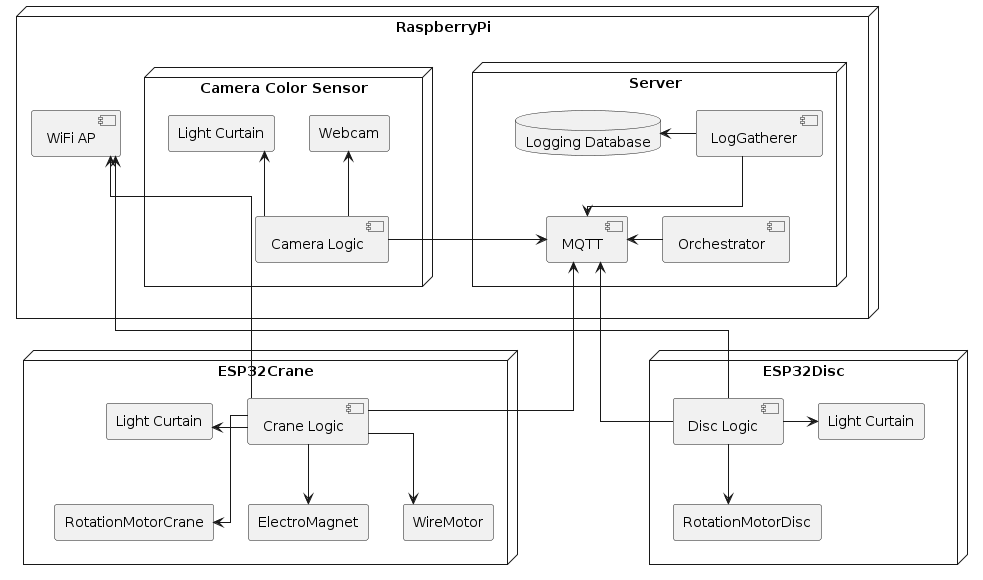
\includegraphics[width=0.5\textwidth]{Image/infrastructure-v3.png}
    \caption{Overview of the system and all its components.}
    \label{fig:system-overview}
\end{figure}

\section{Factory Language (.fl)}\label{appendix:factory-lang}

\subsection{Metamodel}\label{appendix:metamodel} 

\begin{figure}[H]
    \centering
    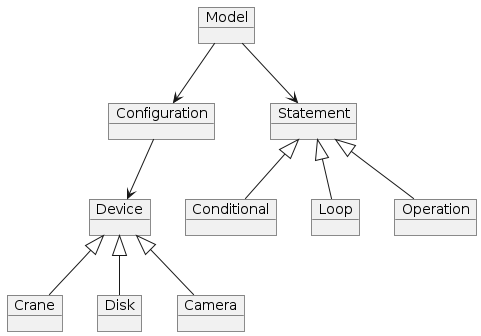
\includegraphics[width=.40\textwidth]{Image/metamodel-final.png}
    \caption{An overview of the metamodel.}
    \label{fig:metamodel}
\end{figure}

\subsection{Grammar Language}\label{appendix:grammar-language}

\begin{minted}[breaklines]{python}
grammar xtext.factoryLang.FactoryLang with org.eclipse.xtext.common.Terminals

generate factoryLang "http://www.factoryLang.xtext/FactoryLang"

Model:
	configurations+=Configuration+ statements+=Statement+;

// ----- CONFIGURATION ----- //
Configuration:
	'create' device=Device;

Device:
	Crane | Disk | Camera;

// ----- CONFIGURATION:CRANE ----- //
Crane returns Device:
	{Crane} 'crane' 'named' name=ID BEGIN targets+=CraneParameter+ END;

CraneParameter returns Parameter:
	CranePositionParameter;

CranePositionParameter returns CraneParameter:
	{CranePositionParameter} 'with' 'position' 'at' degree=INT 'named' name=ID;

// ----- CONFIGURATION:DISK ----- //
Disk returns Device:
	{Disk} 'disk' 'named' name=ID BEGIN slotParameter=DiskSlotParameter targets+=DiskParameter+ END;

DiskParameter returns Parameter:
	DiskZoneParameter;

DiskSlotParameter returns DiskParameter:
	{DiskSlotParameter} 'with' size=INT 'slots';

DiskZoneParameter returns DiskParameter:
	{DiskZoneParameter} 'with' 'zone' 'named' name=ID 'at' 'slot' slot=INT;

// ----- CONFIGURATION:CAMERA ----- //
Camera returns Device:
	{Camera} 'camera' 'named' name=ID BEGIN targets+=CameraParameter+ END;

CameraParameter returns Parameter:
	CameraColorParameter;

CameraColorParameter returns CameraParameter:
	{CameraColorParameter} 'with' 'scannable' 'color' color=COLOR;

// ----- STATEMENTS ----- //
Statement:
	Conditional | Operation | Loop;

// ----- STATEMENTS:CONDITIONALS ----- //
Conditional returns Statement:
	DeviceConditional | VariableConditional;

DeviceConditional returns Conditional:
	{DeviceConditional} 'if' 'device' device=[Device] 'is' (not_operator='not')? ('at')?
	deviceValue=DeviceValue
	'then' BEGIN statements+=Statement* END;

VariableConditional returns Conditional:
	{VariableConditional} 'if' 'variable' variable=[Variable] 'is'
	(comparison_operator=COMPARISON_OPERATOR)?
	variableValue=VariableValue
	'then' BEGIN statements+=Statement* END;

// ----- STATEMENTS:OPERATIONS ----- //
Operation returns Statement:
	CraneOperation | DiskOperation | CameraOperation;

// ----- STATEMENTS:OPERATIONS:CRANE ----- //
CraneOperation returns Operation:
	CranePickupOperation | CraneDropOperation;

CranePickupOperation returns CraneOperation:
	{CranePickupOperation} device=[Crane] 'pickup' 'item' 'at' target=[CraneParameter];

CraneDropOperation returns CraneOperation:
	{CraneDropOperation} device=[Crane] 'drop' 'item' 'at' target=[CraneParameter];

// ----- STATEMENTS:OPERATIONS:DISK ----- //
DiskOperation returns Operation:
	DiskMoveEmptySlotOperation | DiskMoveVariableSlotOperation | DiskMoveSlotOperation | DiskMarkSlotOperation;

DiskMoveSlotOperation returns DiskOperation:
	{DiskMoveSlotOperation} device=[Disk] 'move' 'slot' 'at' source=[DiskZoneParameter] 'to'
	target=[DiskZoneParameter];

DiskMoveVariableSlotOperation returns DiskOperation:
	{DiskMoveVariableSlotOperation} device=[Disk] 'move' 'slot' 'of' variable=[Variable] 'to'
	target=[DiskZoneParameter];

DiskMoveEmptySlotOperation returns DiskOperation:
	{DiskMoveEmptySlotOperation} device=[Disk] 'move' 'empty' 'slot' 'to' target=[DiskZoneParameter];

DiskMarkSlotOperation returns DiskOperation:
	{DiskMarkSlotOperation} device=[Disk] 'mark' 'slot' 'at' target=[DiskZoneParameter] 'as'
	diskSlotValue=DiskSlotValue ('in' quantity=INT measure=TIME)?;

// ----- STATEMENTS:OPERATIONS:CAMERA ----- //
CameraOperation returns Operation:
	CameraScanOperation;

CameraScanOperation returns CameraOperation:
	{CameraScanOperation} device=[Camera] 'scan' 'color' 'into' variable=GlobalVariable;

// ----- STATEMENTS:LOOPS ----- //
Loop returns Statement:
	ForEach;

// ----- STATEMENTS:LOOPS:FOREACH ----- //
ForEach returns Loop:
	{ForEach} 'for' 'each' variable=LocalVariable 'in' device=[Device] 'that' 'is' (operator='not')?
	variableValue=VariableValue
	'then' BEGIN statements+=Statement* END;

// ----- VARIABLES ----- //
LocalVariable returns Variable:
	{LocalVariable} name=ID;

GlobalVariable returns Variable:
	{GlobalVariable} name=ID;

// ----- VALUE TYPES ----- //
DeviceValue:
	value=DiskStateValue | value=ColorValue | ref=[Parameter];

DiskSlotValue:
	value=DiskSlotStateValue | value=ColorValue | ref=[Variable];

VariableValue:
	value=DiskSlotStateValue | value=ColorValue | value=Number | value=DiskStateValue | ref=[Variable];

// ----- VALUE TYPES:ACTUAL VALUES ----- //

DiskStateValue:
	value=DISK_STATES;

DiskSlotStateValue:
 	value=DISK_SLOT_STATES;

ColorValue:
	value=COLOR;

Number:
	value=INT;

// ----- SHARED ENUMS ----- //
enum COMPARISON_OPERATOR:
	UNDEFINED='undefined' | LESS_THAN='less than' | GREATER_THAN='greater than' | NOT='not';

enum COLOR:
	RED='red' | GREEN='green' | BLUE='blue';

enum DISK_SLOT_STATES:
	FREE='free' | IN_PROGRESS='in_progress' | COMPLETE='complete';

enum DISK_STATES:
	FULL='full' | EMPTY='empty';

enum TIME:
	SECONDS='seconds' | SECOND='second' | MINUTES='minutes' | MINUTE='minute' | HOURS='hours' | HOUR='hour';

// ----- TERMINALS ----- //
terminal BEGIN:
	'synthetic:BEGIN';

terminal END:
	'synthetic:END';
\end{minted}

\subsection{Example Factory Language program}\label{appendix:fl}
\begin{minted}[breaklines]{python}
create crane named crane1  
	with position at 0 named pickup 
	with position at 30 named outRed 
	with position at 60 named outGreen 
	with position at 90 named outBlue  

create disk named disk1
	with 8 slots
	with zone named craneZone  at slot 1 
	with zone named cameraZone at slot 3 
	with zone named intakeZone at slot 6 

create camera named camera1  
	with scannable color blue 
	with scannable color green 
	with scannable color red

for each diskSlot in disk1 that is complete then
	disk1 move slot of diskSlot to craneZone
	crane1 pickup item at pickup
	if variable diskSlot is red then  
		crane1 drop item at outRed
	if variable diskSlot is green then  
		crane1 drop item at outGreen
	if variable diskSlot is blue then  
		crane1 drop item at outBlue
	disk1 mark slot at craneZone as free

if device disk1 is not full then  
	disk1 move empty slot to intakeZone
	disk1 mark slot at intakeZone as in_progress 
	disk1 move slot at intakeZone to cameraZone
	camera1 scan color into currentItemColor 
	disk1 mark slot at cameraZone as currentItemColor  
	if variable currentItemColor is red then  
		disk1 mark slot at cameraZone as complete in 10 seconds
	if variable currentItemColor is green then  
		disk1 mark slot at cameraZone as complete in 20 seconds  
	if variable currentItemColor is blue then  
		disk1 mark slot at cameraZone as complete in 30 seconds
\end{minted}


\section{Factory Language (.fl) Updated}\label{appendix:factory-lang-updated}

\subsection{Metamodel}\label{appendix:metamodel-updated} 

\begin{figure}[H]
    \centering
    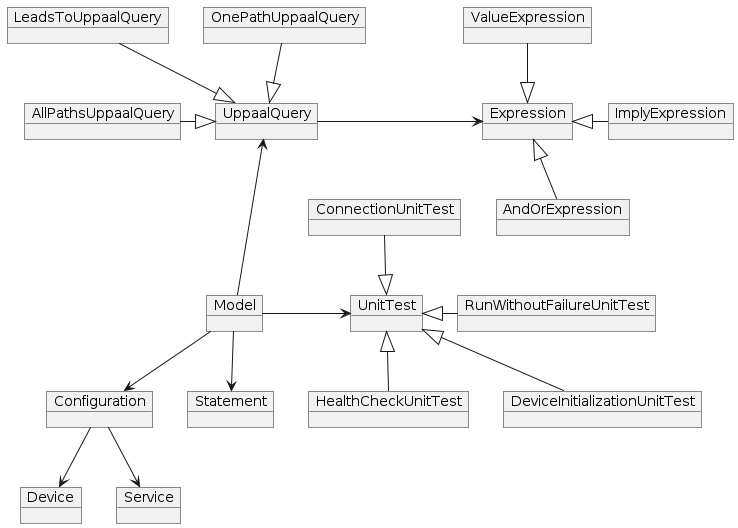
\includegraphics[width=.40\textwidth]{Image/metamodel-individual.png}
    \caption{An overview of the updated metamodel.}
    \label{fig:metamodel-updated}
\end{figure}

\subsection{Grammar Language}\label{appendix:grammar-language-updated}

\begin{minted}[breaklines]{python}
grammar xtext.factoryLang.FactoryLang with org.eclipse.xtext.common.Terminals

generate factoryLang "http://www.factoryLang.xtext/FactoryLang"

Model:
	'init' 'system' 'named' name=ID
	'CONFIGURATION:'
	BEGIN
	configuration=Configuration
	END
	'LOGIC:'
	BEGIN
	statements+=Statement*
	END
	'UNIT TESTS:'
	BEGIN
	unitTests+=UnitTest*
	END
	'UPPAAL QUERIES:'
	BEGIN
	uppaalQueries+=UppaalQuery*
	END;

// uppaalQueries+=UppaalQuery+;
// ----- CONFIGURATION ----- //
Configuration:
	{Configuration} services+=Service* devices+=Device*;

// ----- CONFIGURATION:SERVICE ----- //
Service:
	'define' serviceName=SERVICE_NAME 'named' name=ID 'with' address=Address ':' port=INT;

Address:
	ID ('.' ID)*;

// ----- CONFIGURATION:DEVICE ----- //
Device:
	'create' (Crane | Disk | Camera);

// ----- CONFIGURATION:CRANE ----- //
Crane returns Device:
	{Crane} 'crane' 'named' name=ID BEGIN targets+=CraneParameter+ END;

CraneParameter returns Parameter:
	CranePositionParameter;

CranePositionParameter returns CraneParameter:
	{CranePositionParameter} 'with' 'position' 'at' degree=INT 'named' name=ID;

// ----- CONFIGURATION:DISK ----- //
Disk returns Device:
	{Disk} 'disk' 'named' name=ID BEGIN slotParameter=DiskSlotParameter targets+=DiskParameter+ END;

DiskParameter returns Parameter:
	DiskZoneParameter;

DiskSlotParameter returns DiskParameter:
	{DiskSlotParameter} 'with' size=INT 'slots';

DiskZoneParameter returns DiskParameter:
	{DiskZoneParameter} 'with' 'zone' 'named' name=ID 'at' 'slot' slot=INT;

// ----- CONFIGURATION:CAMERA ----- //
Camera returns Device:
	{Camera} 'camera' 'named' name=ID BEGIN targets+=CameraParameter+ END;

CameraParameter returns Parameter:
	CameraColorParameter;

CameraColorParameter returns CameraParameter:
	{CameraColorParameter} 'with' 'scannable' 'color' color=COLOR;

// ----- STATEMENTS ----- //
Statement:
	Conditional | Operation | Loop;

// ----- STATEMENTS:CONDITIONALS ----- //
Conditional returns Statement:
	DeviceConditional | VariableConditional;

DeviceConditional returns Conditional:
	{DeviceConditional} 'if' 'device' device=[Device] 'is' (not_operator='not')? ('at')?
	deviceValue=DeviceValue
	'then' BEGIN statements+=Statement* END;

VariableConditional returns Conditional:
	{VariableConditional} 'if' 'variable' variable=[Variable] 'is'
	(comparison_operator=COMPARISON_OPERATOR)?
	variableValue=VariableValue
	'then' BEGIN statements+=Statement* END;

// ----- STATEMENTS:OPERATIONS ----- //
Operation returns Statement:
	CraneOperation | DiskOperation | CameraOperation;

// ----- STATEMENTS:OPERATIONS:CRANE ----- //
CraneOperation returns Operation:
	CranePickupOperation | CraneDropOperation;

CranePickupOperation returns CraneOperation:
	{CranePickupOperation} device=[Crane] 'pickup' 'item' 'at' target=[CraneParameter];

CraneDropOperation returns CraneOperation:
	{CraneDropOperation} device=[Crane] 'drop' 'item' 'at' target=[CraneParameter];

// ----- STATEMENTS:OPERATIONS:DISK ----- //
DiskOperation returns Operation:
	DiskMoveEmptySlotOperation | DiskMoveVariableSlotOperation | DiskMoveSlotOperation | DiskMarkSlotOperation |
	DiskWaitOperation;

DiskMoveSlotOperation returns DiskOperation:
	{DiskMoveSlotOperation} device=[Disk] 'move' 'slot' 'at' source=[DiskZoneParameter] 'to'
	target=[DiskZoneParameter];

DiskMoveVariableSlotOperation returns DiskOperation:
	{DiskMoveVariableSlotOperation} device=[Disk] 'move' 'slot' 'of' variable=[Variable] 'to'
	target=[DiskZoneParameter];

DiskMoveEmptySlotOperation returns DiskOperation:
	{DiskMoveEmptySlotOperation} device=[Disk] 'move' 'empty' 'slot' 'to' target=[DiskZoneParameter];

DiskMarkSlotOperation returns DiskOperation:
	{DiskMarkSlotOperation} device=[Disk] 'mark' 'slot' 'at' target=[DiskZoneParameter] 'as'
	diskSlotValue=DiskSlotValue ('in' quantity=INT measure=TIME)?;

DiskWaitOperation returns DiskOperation:
	{DiskWaitOperation} device=[Disk] 'wait' 'for' 'new' 'item';

// ----- STATEMENTS:OPERATIONS:CAMERA ----- //
CameraOperation returns Operation:
	CameraScanOperation;

CameraScanOperation returns CameraOperation:
	{CameraScanOperation} device=[Camera] 'scan' 'color' 'into' variable=GlobalVariable;

// ----- STATEMENTS:LOOPS ----- //
Loop returns Statement:
	ForEach;

// ----- STATEMENTS:LOOPS:FOREACH ----- //
ForEach returns Loop:
	{ForEach} 'for' 'each' variable=LocalVariable 'in' device=[Device] 'that' 'is' (operator='not')?
	variableValue=VariableValue
	'then' BEGIN statements+=Statement* END;

// ----- UnitTests ----- //
UnitTest:
	HealthCheckUnitTest | ConnectionUnitTest | DeviceInitializationUnitTest | RunWithoutFailureUnitTest;

HealthCheckUnitTest returns UnitTest:
	{HealthCheckUnitTest} 'test' service=[Service] 'and' 'assert' 'health status' 'is' status=STATUS;

ConnectionUnitTest returns UnitTest:
	{ConnectionUnitTest} 'test' service=[Service] 'and' 'assert' 'connection' 'is' status=STATUS;

DeviceInitializationUnitTest returns UnitTest:
	{DeviceInitializationUnitTest} 'test' devices+=[Device] (',' devices+=[Device])* 'and' 'assert' ('device' |
	'devices') ('is' | 'are') 'initialized';

RunWithoutFailureUnitTest returns UnitTest:
	{RunWithoutFailureUnitTest} 'test' application=[Model] 'and' 'assert' 'it' 'runs';

// ----- UppaalQueries ----- //
UppaalQuery:
	AllPathsUppaalQuery | OnePathUppaalQuery | LeadsToUppaalQuery;

AllPathsUppaalQuery returns UppaalQuery:
	{AllPathsUppaalQuery} 'query' 'that' property=('forever' | 'eventually') 'on' 'all' 'paths' '(' BEGIN not=('not')?
	expression=AndOrExpression END ')';

OnePathUppaalQuery returns UppaalQuery:
	{OnePathUppaalQuery} 'query' 'that' property=('forever' | 'eventually') 'on' 'one' 'path' '(' BEGIN not=('not')?
	expression=AndOrExpression END ')';

LeadsToUppaalQuery returns UppaalQuery:
	{LeadsToUppaalQuery} 'query' 'that' '(' BEGIN not1=('not')? stateOne=ValueExpression 'leads' 'to' not2=('not')?
	stateTwo=ValueExpression END ')';

AndOrExpression returns Expression:
	ImplyExpression (({Or.left=current} 'or' | {And.left=current} 'and') not=('not')? right=ImplyExpression)*;

ImplyExpression returns Expression:
	ValueExpression (({Imply.left=current} 'imply') not=('not')? right=ValueExpression)*;

ValueExpression returns Expression:
	{Parenthesis} '(' parenthesizedExpression=AndOrExpression ')' | DeviceState;

DeviceState:
	device=[Device] '.' location=ID;

// ----- VARIABLES ----- //
LocalVariable returns Variable:
	{LocalVariable} name=ID;

GlobalVariable returns Variable:
	{GlobalVariable} name=ID;

// ----- VALUE TYPES ----- //
DeviceValue:
	value=DiskStateValue | value=ColorValue | ref=[Parameter];

DiskSlotValue:
	value=DiskSlotStateValue | value=ColorValue | ref=[Variable];

VariableValue:
	value=DiskSlotStateValue | value=ColorValue | value=Number | value=DiskStateValue | ref=[Variable];

// ----- VALUE TYPES:ACTUAL VALUES ----- //
DiskStateValue:
	value=DISK_STATES;

DiskSlotStateValue:
	value=DISK_SLOT_STATES;

ColorValue:
	value=COLOR;

Number:
	value=INT;

// ----- SHARED ENUMS ----- //
enum COMPARISON_OPERATOR:
	UNDEFINED='undefined' | LESS_THAN='less than' | GREATER_THAN='greater than' | NOT='not';

enum COLOR:
	RED='red' | GREEN='green' | BLUE='blue';

enum DISK_SLOT_STATES:
	FREE='free' | IN_PROGRESS='in_progress' | COMPLETE='complete';

enum DISK_STATES:
	FULL='full' | EMPTY='empty';

enum TIME:
	SECONDS='seconds' | SECOND='second' | MINUTES='minutes' | MINUTE='minute' | HOURS='hours' | HOUR='hour';

enum SERVICE_NAME:
	MQTT='mqtt' | DATABASE='database';

enum STATUS:
	UP='up' | DOWN='down';

// ----- TERMINALS ----- //
terminal BEGIN:
	'synthetic:BEGIN';

terminal END:
	'synthetic:END';
\end{minted}

\subsection{Example Factory Language program}\label{appendix:fl-updated}
\begin{minted}[breaklines]{python}
init system named OrchestratorService

CONFIGURATION:
	define mqtt named ^mqtt with ^test.mosquitto.org:1883
	define database named influxdb with influxdb.devantler.com:8086
	
	create crane named crane1
		with position at 0 named intake 
		with position at 40 named outRed 
		with position at 55 named outGreen 
		with position at 70 named outBlue  
	
	create disk named disk1
		with 4 slots
		with zone named craneZone  at slot 1 
		with zone named cameraZone at slot 2
		with zone named intakeZone at slot 3 
	
	create camera named camera1
		with scannable color blue 
		with scannable color green 
		with scannable color red

LOGIC:
	for each diskSlot in disk1 that is complete then
		disk1 move slot of diskSlot to craneZone
		crane1 pickup item at intake
		disk1 mark slot at craneZone as free
		if variable diskSlot is red then  
			crane1 drop item at outRed
		if variable diskSlot is green then  
			crane1 drop item at outGreen
		if variable diskSlot is blue then  
			crane1 drop item at outBlue
	
	if device disk1 is not full then  
		disk1 move empty slot to intakeZone
		disk1 wait for new item
		disk1 mark slot at intakeZone as in_progress 
		disk1 move slot at intakeZone to cameraZone
		camera1 scan color into currentItemColor 
		disk1 mark slot at cameraZone as currentItemColor  
		if variable currentItemColor is red then  
			disk1 mark slot at cameraZone as complete in 10 seconds  
		if variable currentItemColor is green then  
			disk1 mark slot at cameraZone as complete in 20 seconds  
		if variable currentItemColor is blue then  
			disk1 mark slot at cameraZone as complete in 30 seconds

UNIT TESTS:
	test ^mqtt and assert health status is up
	test ^mqtt and assert connection is up
	test influxdb and assert health status is down
	test influxdb and assert connection is down
	test camera1, crane1, disk1 and assert devices are initialized
	test OrchestratorService and assert it runs
	
UPPAAL QUERIES:
	//A[] (disk1.Position1 imply (disk1.Position1 or disk1.Position2 or disk1.Position3))
	query that forever on all paths (
		disk1.Position1 imply (disk1.Position1 or disk1.Position2 or disk1.Position3)
	)
	
	//A<> (disk1.Stopped and crane1.crane1_Stopped) imply (disk1.Position1 and crane1.crane1_Stopped)
	query that eventually on all paths (
		(disk1.Stopped and crane1.Stopped) imply (disk1.Position1 and crane1.Stopped)
	)
	
	//E[] (disk1.Position1 or disk1.Position2 or disk1.Position3 or disk1.Position4)
	query that forever on one path (
		disk1.Position1 or disk1.Position2 or disk1.Position3 or disk1.Position4
	)
	
	//E<> (disk1.Position1 imply disk1.Position2)
	query that eventually on one path (
		disk1.Position1 imply disk1.Position2
	)
	
	//camera1.camera1_Green --> camera1.camera1_Idle
	query that (
		camera1.camera1_Green leads to camera1.camera1_Idle
	)
	
	//Just a test to show negation works
	query that eventually on all paths (
		not camera1.dsd or not disk1.sds
	)
\end{minted}

\section{The Orchestrator}\label{appendix:orchestrator}

\subsection{Program.cs}

\begin{minted}[breaklines]{csharp}
using System;
using Entities;
using Mqtt;

#region Variables
IMqttService mqtt = new MqttService();

Dictionary<string, Crane> cranes = new();
Dictionary<string, Disk> disks = new();
Dictionary<string, Camera> cameras = new();

bool running = true;
#endregion

#region Main
Setup();
Run().GetAwaiter().GetResult();
#endregion

void Setup()
{
    cranes.Add("crane1", new Crane("crane1", new Dictionary<string, int>()
    {
        {"intake", 0},
        {"outRed", 40},
        {"outGreen", 55},
        {"outBlue", 70}
    }, mqtt));

    disks.Add("disk1", new Disk("disk1", 8, new Dictionary<string, int>()
    {
        {"craneZone", 0},
        {"cameraZone", 4},
        {"intakeZone", 2}
    }, mqtt));

    cameras.Add("camera1", new Camera("camera1", new List<string>()
    {
        "blue",
        "green",
        "red"
    }, mqtt));
}

async Task Run()
{
    var crane1 = cranes["crane1"];
    var disk1 = disks["disk1"];
    var camera1 = cameras["camera1"];

    while (running)
    {
        foreach (var diskSlot in disk1.GetSlotsWithMark(SlotState.Complete))
        {
            await disk1.MoveSlot(diskSlot.Number, "craneZone");
            await crane1.GoTo("intake");
            await crane1.PickupItem();
            if (diskSlot.HasMark("RED"))
            {
                await crane1.GoTo("outRed");
                await crane1.DropItem();
            }
            if (diskSlot.HasMark("GREEN"))
            {
                await crane1.GoTo("outGreen");
                await crane1.DropItem();
            }
            if (diskSlot.HasMark("BLUE"))
            {
                await crane1.GoTo("outBlue");
                await crane1.DropItem();
            }
            disk1.MarkSlot(diskSlot.Number, SlotState.Empty);
        }
        if (!disk1.IsFull())
        {
            var currentSlot = disk1.GetEmptySlotNumber();
            await disk1.MoveSlot(currentSlot, "intakeZone");
            Console.WriteLine($"Empty slot: {currentSlot}");
            await disk1.WaitForIntake();
            disk1.MarkSlot(currentSlot, SlotState.InProgress);
            await disk1.MoveZoneToZone("intakeZone", "cameraZone");
            var currentItemColor = await camera1.Scan() ?? "RED";
            disk1.MarkSlot(currentSlot, currentItemColor);
            if (currentItemColor == "RED")
            {
                Task.Run(async () =>
                {
                    var slotNo = currentSlot;
                    await Task.Delay(3 * 90 * 1000);
                    disk1.MarkSlot(slotNo, SlotState.Complete);
                });
            }
            if (currentItemColor == "GREEN")
            {
                Task.Run(async () =>
                {
                    var slotNo = currentSlot;
                    await Task.Delay(2 * 90 * 1000);
                    disk1.MarkSlot(slotNo, SlotState.Complete);
                });
            }
            if (currentItemColor == "BLUE")
            {
                Task.Run(async () =>
                {
                    var slotNo = currentSlot;
                    await Task.Delay(4 * 60 * 1000);
                    disk1.MarkSlot(slotNo, SlotState.Complete);
                });
            }
        }
    }
}
\end{minted}

\subsection{Dockerfile}

\begin{minted}[breaklines]{dockerfile}
FROM mcr.microsoft.com/dotnet/runtime:6.0 AS final
WORKDIR /app
ARG TARGETARCH
ADD ./${TARGETARCH}.tar /app
ENTRYPOINT ["dotnet", "OrchestratorService.dll"]
\end{minted}

\begin{minted}[breaklines]{dockerfile}
FROM mcr.microsoft.com/dotnet/runtime:6.0 AS final
WORKDIR /app
ARG TARGETARCH
ADD ./${TARGETARCH}.tar /app
ENTRYPOINT ["dotnet", "OrchestratorService.dll"]
\end{minted}

\subsection{GitHub Action}

\begin{minted}[breaklines]{yaml}
name: Push Orchestrator image to ghcr

on:
  push:
    branches: ['main']
    paths:
      - 'SemesterProject/RaspberryPi/ \
        OrchestratorService/**'

jobs:
  build-and-push-image:
    runs-on: ubuntu-latest
    permissions:
      contents: read
      packages: write
    steps:
      - name: Checkout repository
        uses: actions/checkout@v3

      - name: Log in to the Container registry
        uses: docker/login-action@v1
        with:
          registry: ghcr.io
          username: ${{ github.actor }}
          password: ${{ secrets.GITHUB_TOKEN }}

      - name: Build and push
        run: |
          docker buildx create --use
          sh ./SemesterProject/RaspberryPi/ \
                OrchestratorService/build.sh
\end{minted}
\section{The Updated Orchestrator}\label{appendix:orchestrator-updated}

\subsection{Program.cs}\label{appendix:orchestrator-updated-programcs}

\begin{minted}[breaklines]{csharp}
using Entities;
using Mqtt;

namespace OrchestratorService;

public class Program
{
    public IMqttService mqtt = new MqttService();
    
    public Dictionary<string, Crane> cranes = new();
    public Dictionary<string, Disk> disks = new();
    public Dictionary<string, Camera> cameras = new();
    
    public bool running;
    
    private static void Main()
    {
        Program program = new();
        program.Setup();
        program.Run().GetAwaiter().GetResult();
    }
    
    public void Setup()
    {
        cranes.Add("crane1", new Crane("crane1", new Dictionary<string, int>()
        {
            {"intake", 0},
            {"outRed", 40},
            {"outGreen", 55},
            {"outBlue", 70}
        }, mqtt));
    
        disks.Add("disk1", new Disk("disk1", 8, new Dictionary<string, int>()
        {
            {"craneZone", 1},
            {"cameraZone", 2},
            {"intakeZone", 3}
        }, mqtt));
    
        cameras.Add("camera1", new Camera("camera1", new List<string>()
        {
            "blue",
            "green",
            "red"
        }, mqtt));
    }
    
    public async Task Run()	
    {
        var crane1 = cranes["crane1"];
        var disk1 = disks["disk1"];
        var camera1 = cameras["camera1"];
        running = true;
        while (running)
        {
            foreach (var diskSlot in disk1.GetSlotsWithMark(SlotState.Complete))
            {
                await disk1.MoveSlot(diskSlot.Number, "craneZone");
                await crane1.GoTo("intake");
                await crane1.PickupItem();
                disk1.MarkSlot("craneZone", SlotState.Empty);
                if (diskSlot.HasMark("RED"))
                {
                    await crane1.GoTo("outRed");
                    await crane1.DropItem();
                }
                if (diskSlot.HasMark("GREEN"))
                {
                    await crane1.GoTo("outGreen");
                    await crane1.DropItem();
                }
                if (diskSlot.HasMark("BLUE"))
                {
                    await crane1.GoTo("outBlue");
                    await crane1.DropItem();
                }
            }
            if (!disk1.IsFull())
            {
                await disk1.MoveSlot(disk1.GetEmptySlotNumber(), "intakeZone");
                await disk1.WaitForIntake();
                disk1.MarkSlot("intakeZone", SlotState.InProgress);
                await disk1.MoveSlot("intakeZone", "cameraZone");
                var currentItemColor = await camera1.Scan();
                disk1.MarkSlot("cameraZone", currentItemColor);
                if (currentItemColor == "RED")
                {
                    Task.Run(async () =>
                    {
                        await Task.Delay(10000);
                        disk1.MarkSlot("cameraZone", SlotState.Complete);
                    });
                }
                if (currentItemColor == "GREEN")
                {
                    Task.Run(async () =>
                    {
                        await Task.Delay(20000);
                        disk1.MarkSlot("cameraZone", SlotState.Complete);
                    });
                }
                if (currentItemColor == "BLUE")
                {
                    Task.Run(async () =>
                    {
                        await Task.Delay(30000);
                        disk1.MarkSlot("cameraZone", SlotState.Complete);
                    });
                }
            }
        }
    }
}    
\end{minted}

\subsection{Dockerfile}\label{appendix:orchestrator-updated-dockerfile}

\begin{minted}[breaklines]{dockerfile}
FROM mcr.microsoft.com/dotnet/sdk:6.0 AS build
WORKDIR /app
COPY *.sln .
COPY src/OrchestratorService/*.csproj ./src/OrchestratorService/
COPY test/OrchestratorService.Tests/*.csproj ./test/OrchestratorService.Tests/
RUN dotnet restore

COPY . .
RUN dotnet build

FROM build AS testrunner
WORKDIR /app/test/OrchestratorService.Tests
CMD ["dotnet", "test", "--logger:trx"]

FROM build AS test
WORKDIR /app/test/OrchestratorService.Tests
RUN dotnet test --logger:trx

FROM build AS publish
WORKDIR /app/src/OrchestratorService
RUN dotnet publish -c Release -o out

FROM mcr.microsoft.com/dotnet/aspnet:6.0 AS runtime
WORKDIR /app
COPY --from=publish /app/src/OrchestratorService/out ./
EXPOSE 5000
ENTRYPOINT ["dotnet", "OrchestratorService.dll"]
\end{minted}

\subsection{GitHub Action}\label{appendix:orchestrator-updated-githubaction}

\begin{minted}[breaklines]{yaml}
name: Orchestrator Service V3

on:
  push:
    paths:
    - 'SemesterProject/RaspberryPi/OrchestratorService/**'
    - '.github/workflows/orchestrator-service-docker.yml'
    branches:
      - master
    tags:
      - 'v*'
    
jobs:
  build-and-push-image:
    runs-on: ubuntu-latest
    permissions:
      contents: read
      packages: write

    steps:
      - name: Checkout repository
        uses: actions/checkout@v3
              
      - name: Set up QEMU
        uses: docker/setup-qemu-action@v2

      - name: Set up Docker Buildx
        uses: docker/setup-buildx-action@v2
        
      - name: Docker meta
        id: meta
        uses: docker/metadata-action@v4
        with:
          images: ghcr.io/devantler/orchestratorservice
        
      - name: Log in to the Container registry
        uses: docker/login-action@v2
        with:
          registry: ghcr.io
          username: ${{ github.actor }}
          password: ${{ secrets.GITHUB_TOKEN }}
      - name: Run Unit Tests
        run: |
          docker build --target test SemesterProject/RaspberryPi/OrchestratorService/
        continue-on-error: true
      - name: Build and push Docker image
        uses: docker/build-push-action@v3
        with:
          context: SemesterProject/RaspberryPi/OrchestratorService/
          file: SemesterProject/RaspberryPi/OrchestratorService/Dockerfile
          platforms: linux/arm64
          push: true
          tags: ${{ steps.meta.outputs.tags }}
          labels: ${{ steps.meta.outputs.labels }}
\end{minted}
\section{Functional and non-functional requirements}\label{appendix:requirements}

\subsection{Functional requirements}\label{appendix:functional-requirements}
\begin{enumerate}
    \item Functional requirements for the disk.
    \begin{enumerate}
        \item The disk must be able to rotate items from one location to another.
        \item The disk must be able to rotate the shortest path.
        \item The disk must be able to avoid tangling wires while rotating.
        \item The disk must have configurable slots for items.
        \item The disk must have configurable zones for operations, e.g., scanning, crane pick up, intake.
        \item The disk must have a stop function that conforms to danish machine safety standards.
        \item The disk's stop function must halt all movement if the system is in an unsafe state.
        \item The disk's stop function must be able to resume operations when the unsafe condition is resolved.
        \item The disk must have WiFi connectivity.
        \item The disk must be controllable with MQTT.
    \end{enumerate}
    \vspace{1em}
    
    \item Functional requirements for the crane.
    \begin{enumerate}
        \item The crane must be able to rotate its jib from one location to another.
        \item The crane must be able to raise and lower with its hoist.
        \item The crane must be able to pick up and deliver items.
        \item The crane is not allowed to drop items before it reaches its target location.
        \item The crane must be able to rotate the shortest path.
        \item The crane must be able to avoid tangling wires while rotating.
        \item The crane must have a stop function that conforms to danish machine safety standards.
        \item The crane's stop function must halt all movement if the system is in an unsafe state.
        \item The crane's stop function must be able to resume operations when the unsafe condition is resolved.
        \item The crane must have WiFi connectivity.
        \item The crane must be controllable with MQTT.
    \end{enumerate}
    \vspace{1em}


    \item Functional requirements for the camera.
    \begin{enumerate}
        \item The camera must be able scan colors of items.
        \item The camera must be able to retry scanning if it fails.
        \item The camera must have WiFi connectivity.
        \item The camera must be controllable with MQTT.
    \end{enumerate}
\end{enumerate}

\subsection{Non-functional requirements}

\begin{enumerate}
    \item Non-functional requirements for the disk.
    \begin{enumerate}
        \item The disk must operate reliably.
        \item The disk must operate safely and not cause harm to people.
    \end{enumerate}
    \vspace{1em}
    
    \item Non-functional requirements for the crane.
    \begin{enumerate}
        \item The crane must operate reliably.
        \item The crane must operate safely and not cause harm to people.
    \end{enumerate}
    \vspace{1em}
    
    \item Non-functional requirements for the camera.
    \begin{enumerate}
        \item The camera must operate reliably.
    \end{enumerate}
\end{enumerate}


\section{Individual Features - List of Changes}\label{appendix:individual-feature-list-of-changes}

\hypertarget{general}{%
\subsection{General}\label{general}}

\begin{itemize}
\item
  Updated workflow for orchestrator service to include running unit
  tests.
\item
  Updated program.fl
\end{itemize}

\hypertarget{general-grammar}{%
\subsection{General Grammar}\label{general-grammar}}

\begin{itemize}

\item
  Added system initialization so the system has a name
\item
  Changed Model to have a Configuration instead of multiple
  configurations
\item
  Changed Configuration to have a list of services and devices
\item
  Added title separators for configuration, logic, unit tests and Uppaal
  queries.
\end{itemize}

\hypertarget{services-grammar}{%
\subsection{Services Grammar}\label{services-grammar}}

\begin{itemize}
\item
  Added Service grammar rule

  \begin{itemize}
  \item
    Added Mqtt grammar rule
  \item
    Added Database grammar rule
  \item
    Added Address grammar rule
  \end{itemize}
\item
  Changed Device grammar rule to include `create' keyword
\item
  Added enum SERVICE\_NAME to specify supported services.
\end{itemize}

\hypertarget{unit-tests-grammar}{%
\subsection{Unit Tests Grammar}\label{unit-tests-grammar}}

\begin{itemize}
\item
  Added UnitTest grammar rule

  \begin{itemize}
  \item
    Added HealthCheckUnitTest
  \item
    Added ConnectionUnitTest
  \item
    Added DeviceInitializationUnitTest
  \item
    Added RunWithoutFailureUnitTest
  \end{itemize}
\end{itemize}

\hypertarget{uppaal-queries-grammar}{%
\subsection{UPPAAL Queries Grammar}\label{uppaal-queries-grammar}}

\begin{itemize}
\item
  Added UppaalQuery grammar rule

  \begin{itemize}
  \item
    Added AllPathsUppaalQuery
  \item
    Added OnePathUppaalQuery
  \item
    Added LeadsToUppaalQuery
  \end{itemize}
\item
  Added Expression grammar rule with left-factoring

  \begin{itemize}
  \item
    Added AddOrExpression
  \item
    Added ImplyExpression
  \item
    Added ValueExpression
  \item
    Added DeviceState
  \item
    Added Negation
  \end{itemize}
\end{itemize}

\hypertarget{c-code-generation}{%
\subsection{C\# Code generation}\label{c-code-generation}}

\begin{itemize}
\item
  Code generated project title from system name for Orchestrator
\item
  Moved all csharp code generation files to
  \texttt{xtext.factoryLang.generator.csharp}
\item
  Changed code generation of C\# src project so the program is testable.
\item
  Code-Generated solution file
\item
  Added code generation to generate a C\# test project.

  \begin{itemize}
  \item
    Code generated Unit Tests.

    \begin{itemize}
    \item
      Implemented HealthCheckUnitTest
    \item
      Implemented ConnectionUnitTest
    \item
      Implemented DeviceInitializationUnitTest
    \item
      Implemented RunWithoutFailureUnitTest
    \end{itemize}
  \end{itemize}
\item
  Code-Generated Dockerfile that includes src and test projects.
\end{itemize}

\hypertarget{uppaal-code-generation}{%
\subsection{UPPAAL Code Generation}\label{uppaal-code-generation}}

\begin{itemize}
\item
  Moved all UPPAAL code generation files to
  \texttt{xtext.factoryLang.generator.uppaal}
\item
  Code generated system folder name from system name for UPPAAL Project
\item
  Code generated Queries

  \begin{itemize}
  \item
    Implemented AllPathsUppaalQuery
  \item
    Implemented OnePathUppaalQuery
  \item
    Implemented LeadsToUppaalQuery
  \item
    Implemented Negation
  \end{itemize}
\end{itemize}
\onecolumn
\section{Logs Graph}\label{appendix:log-graph}

\begin{figure}[H]
    \centering
    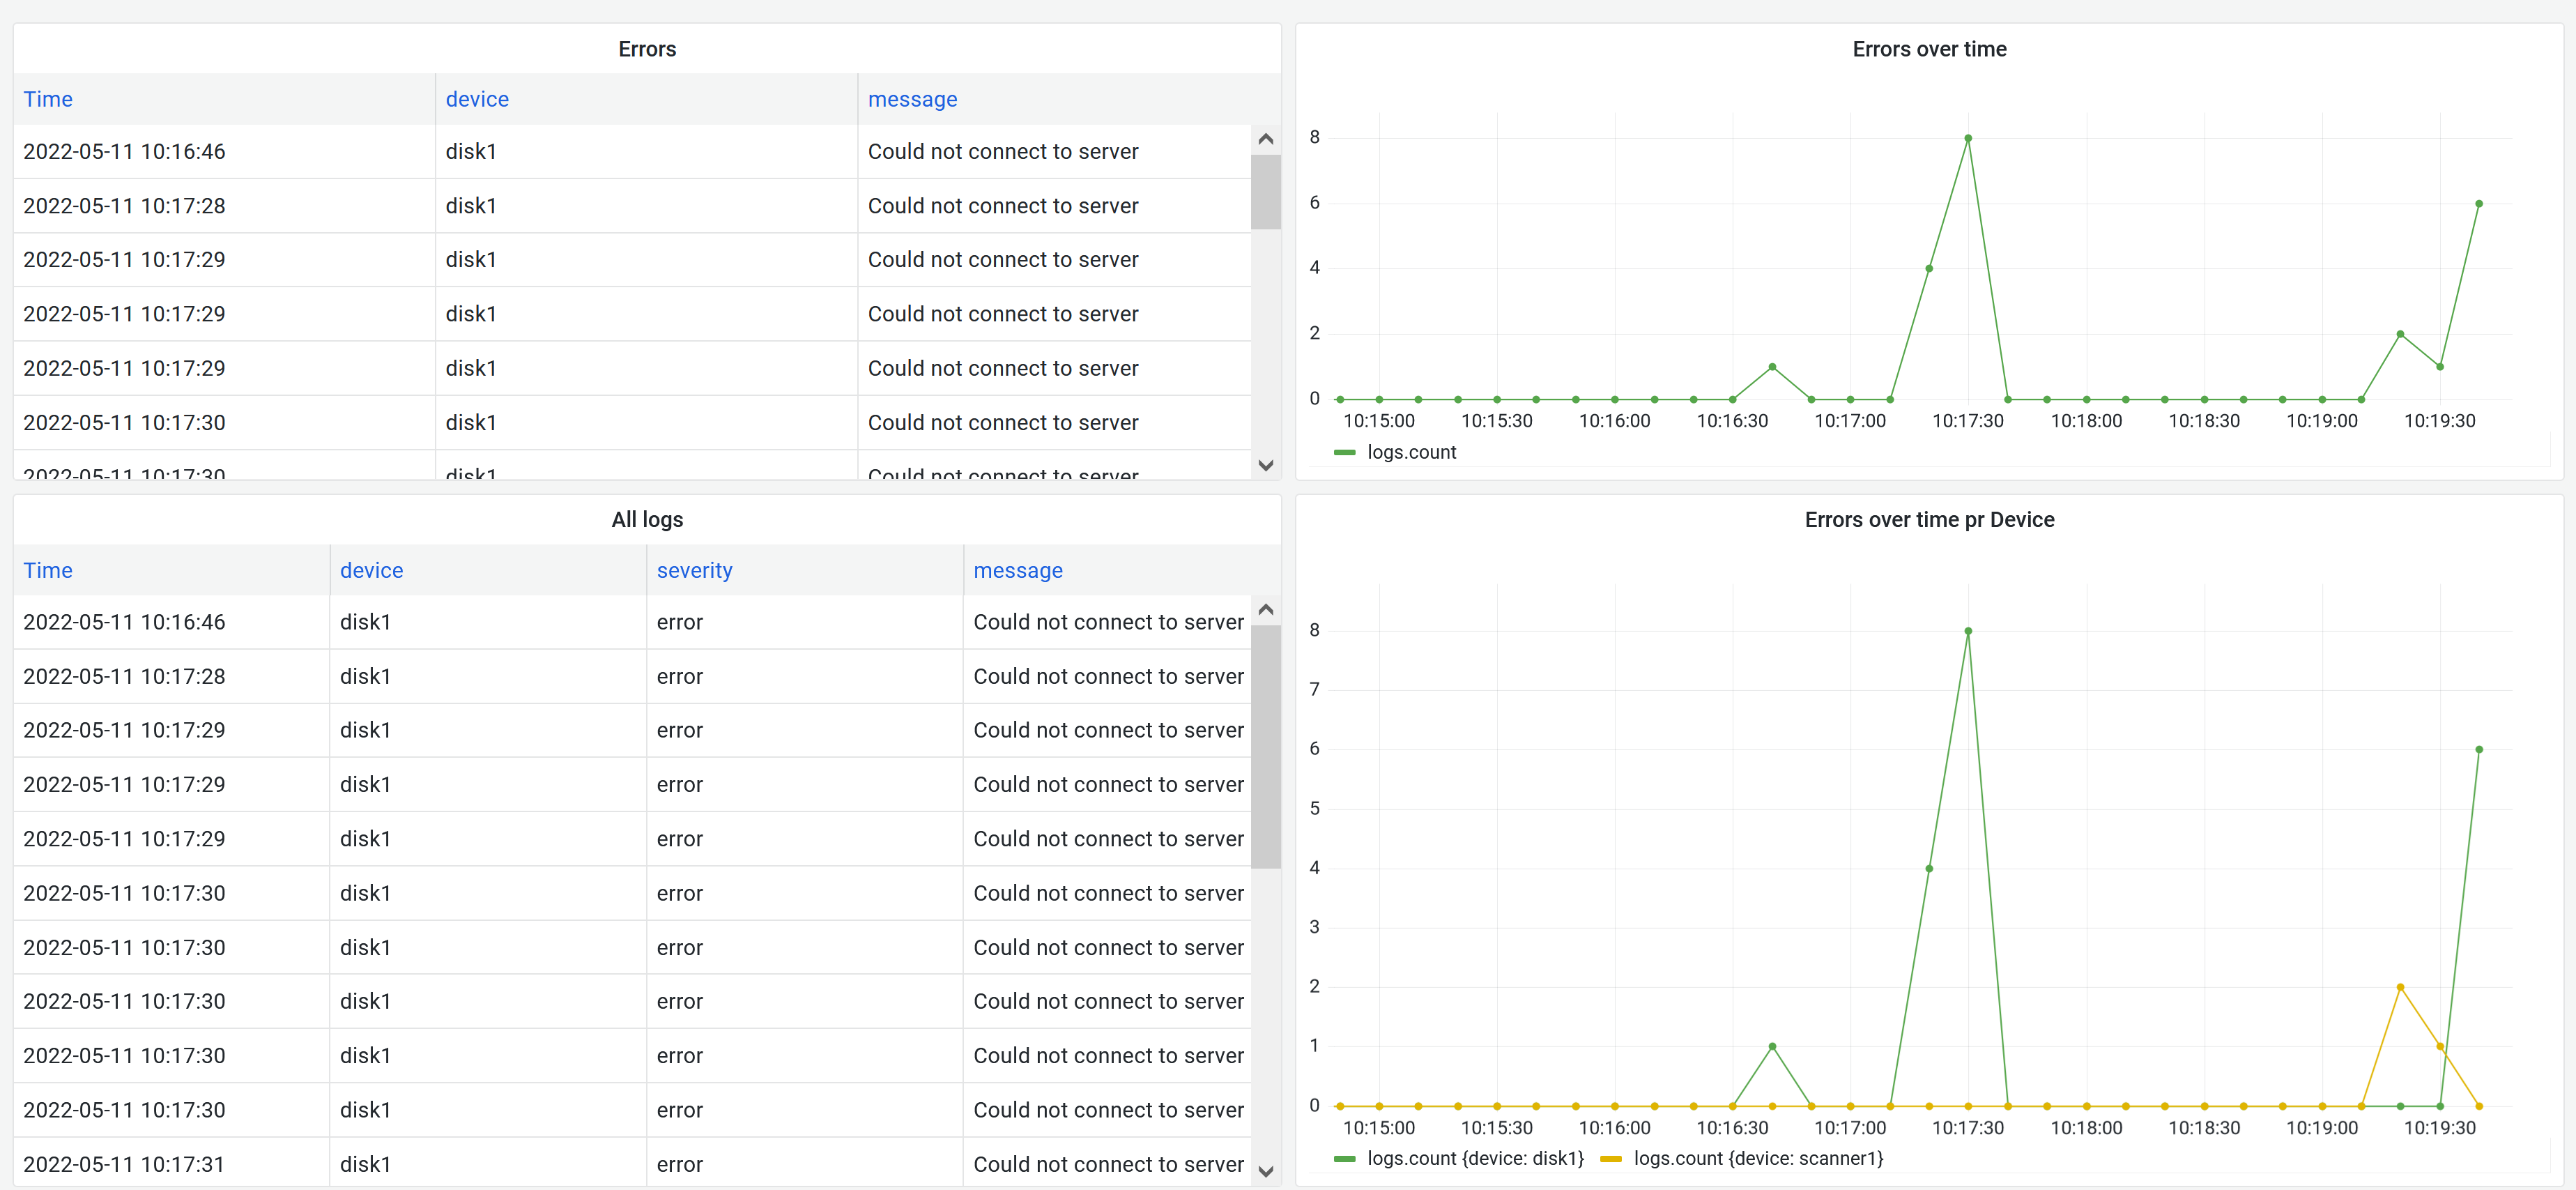
\includegraphics[width=\textwidth]{Image/LoggingGraph.png}
    \caption{Logs graph}
    \label{fig:logs_graph}
\end{figure}
\section{Trustworthy Systems - Course objectives}\label{appendix:course-objectives}

\subsection{Learning objectives - Knowledge}\label{appendix:knowledge}

\begin{itemize}
    \item Obtain an understanding of and explain the topics that are associated with the project.
    \item Obtain an understanding of the elements of engineering projects with a scientific purpose.
\end{itemize}

\subsection{Learning objectives - Skills}\label{appendix:skills}

\begin{itemize}
    \item Identify, analyse and make qualified choices for the design of trustworthy systems given functional and non-functional requirements.
    \item Implement, test and evaluate trustworthy systems in regard to functional and non-functional requirements.
\end{itemize}

\subsection{Learning objectives - Competences}\label{appendix:competences}

\begin{itemize}
    \item Conduct software development within topics that are associated with the project.
    \item Carry out professional engineering use of software technologies in development of software solutions within the topics that are associated with the project.
    \item Work structured and scientifically with engineering solutions to open-ended challenges and disseminate knowledge about the solutions orally and in writing.
\end{itemize}



\onecolumn
\section{Templates}\label{appendix:templates}

\subsection{The Master Controller template}
\begin{figure}[H]
    \centering
    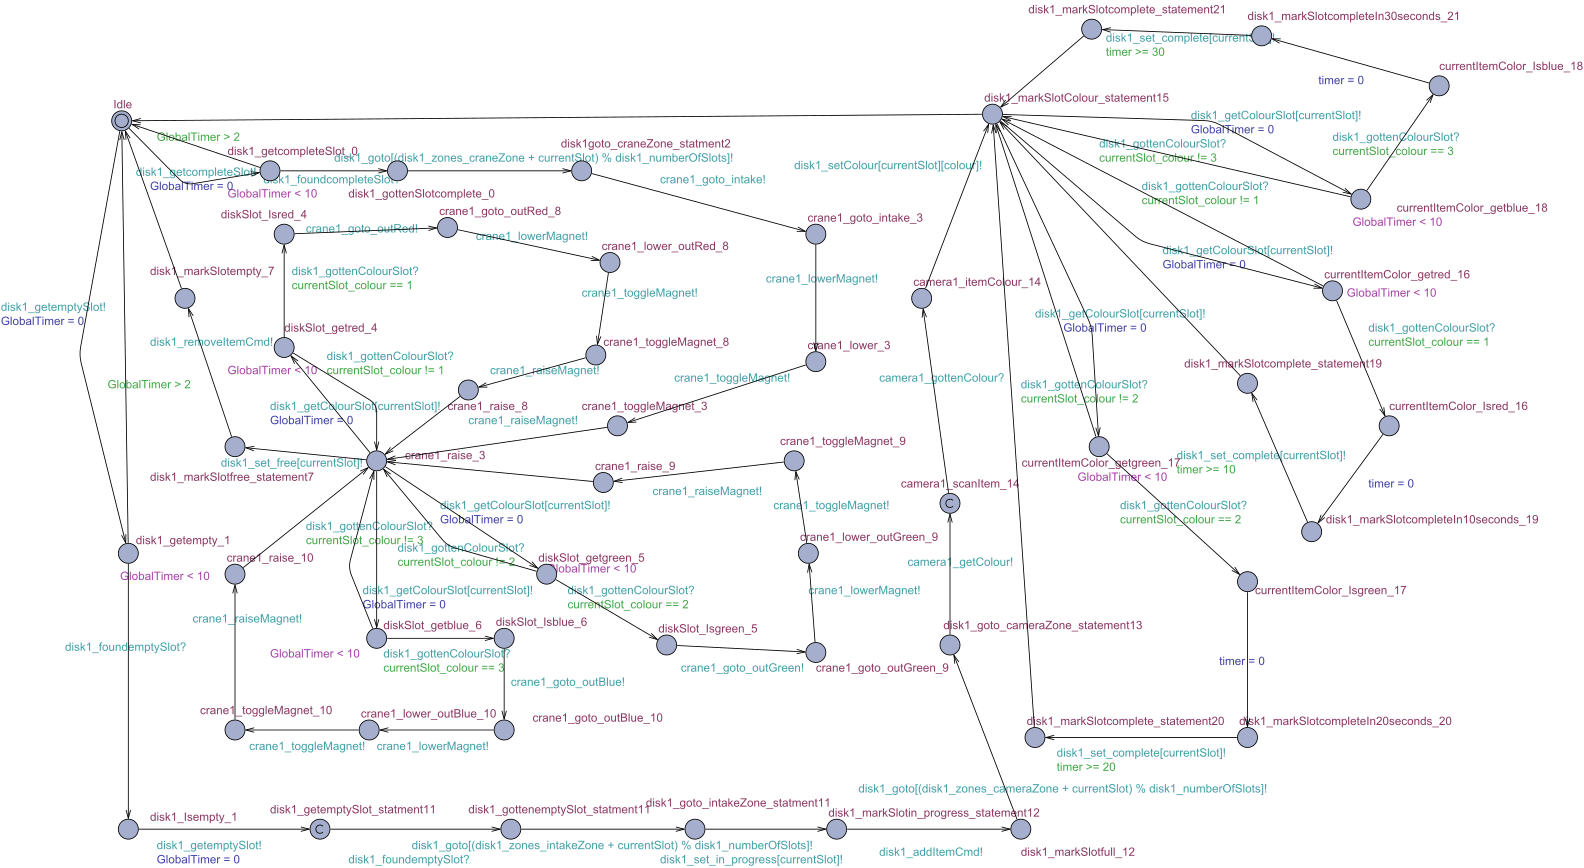
\includegraphics[width=\textwidth]{Image/uppaal-templates/MasterController.png}
    \caption{Master Controller.}
    \label{fig:master_controller}
\end{figure}

\newpage
\subsection{The Disk template}
\begin{figure}[H]
    \centering
    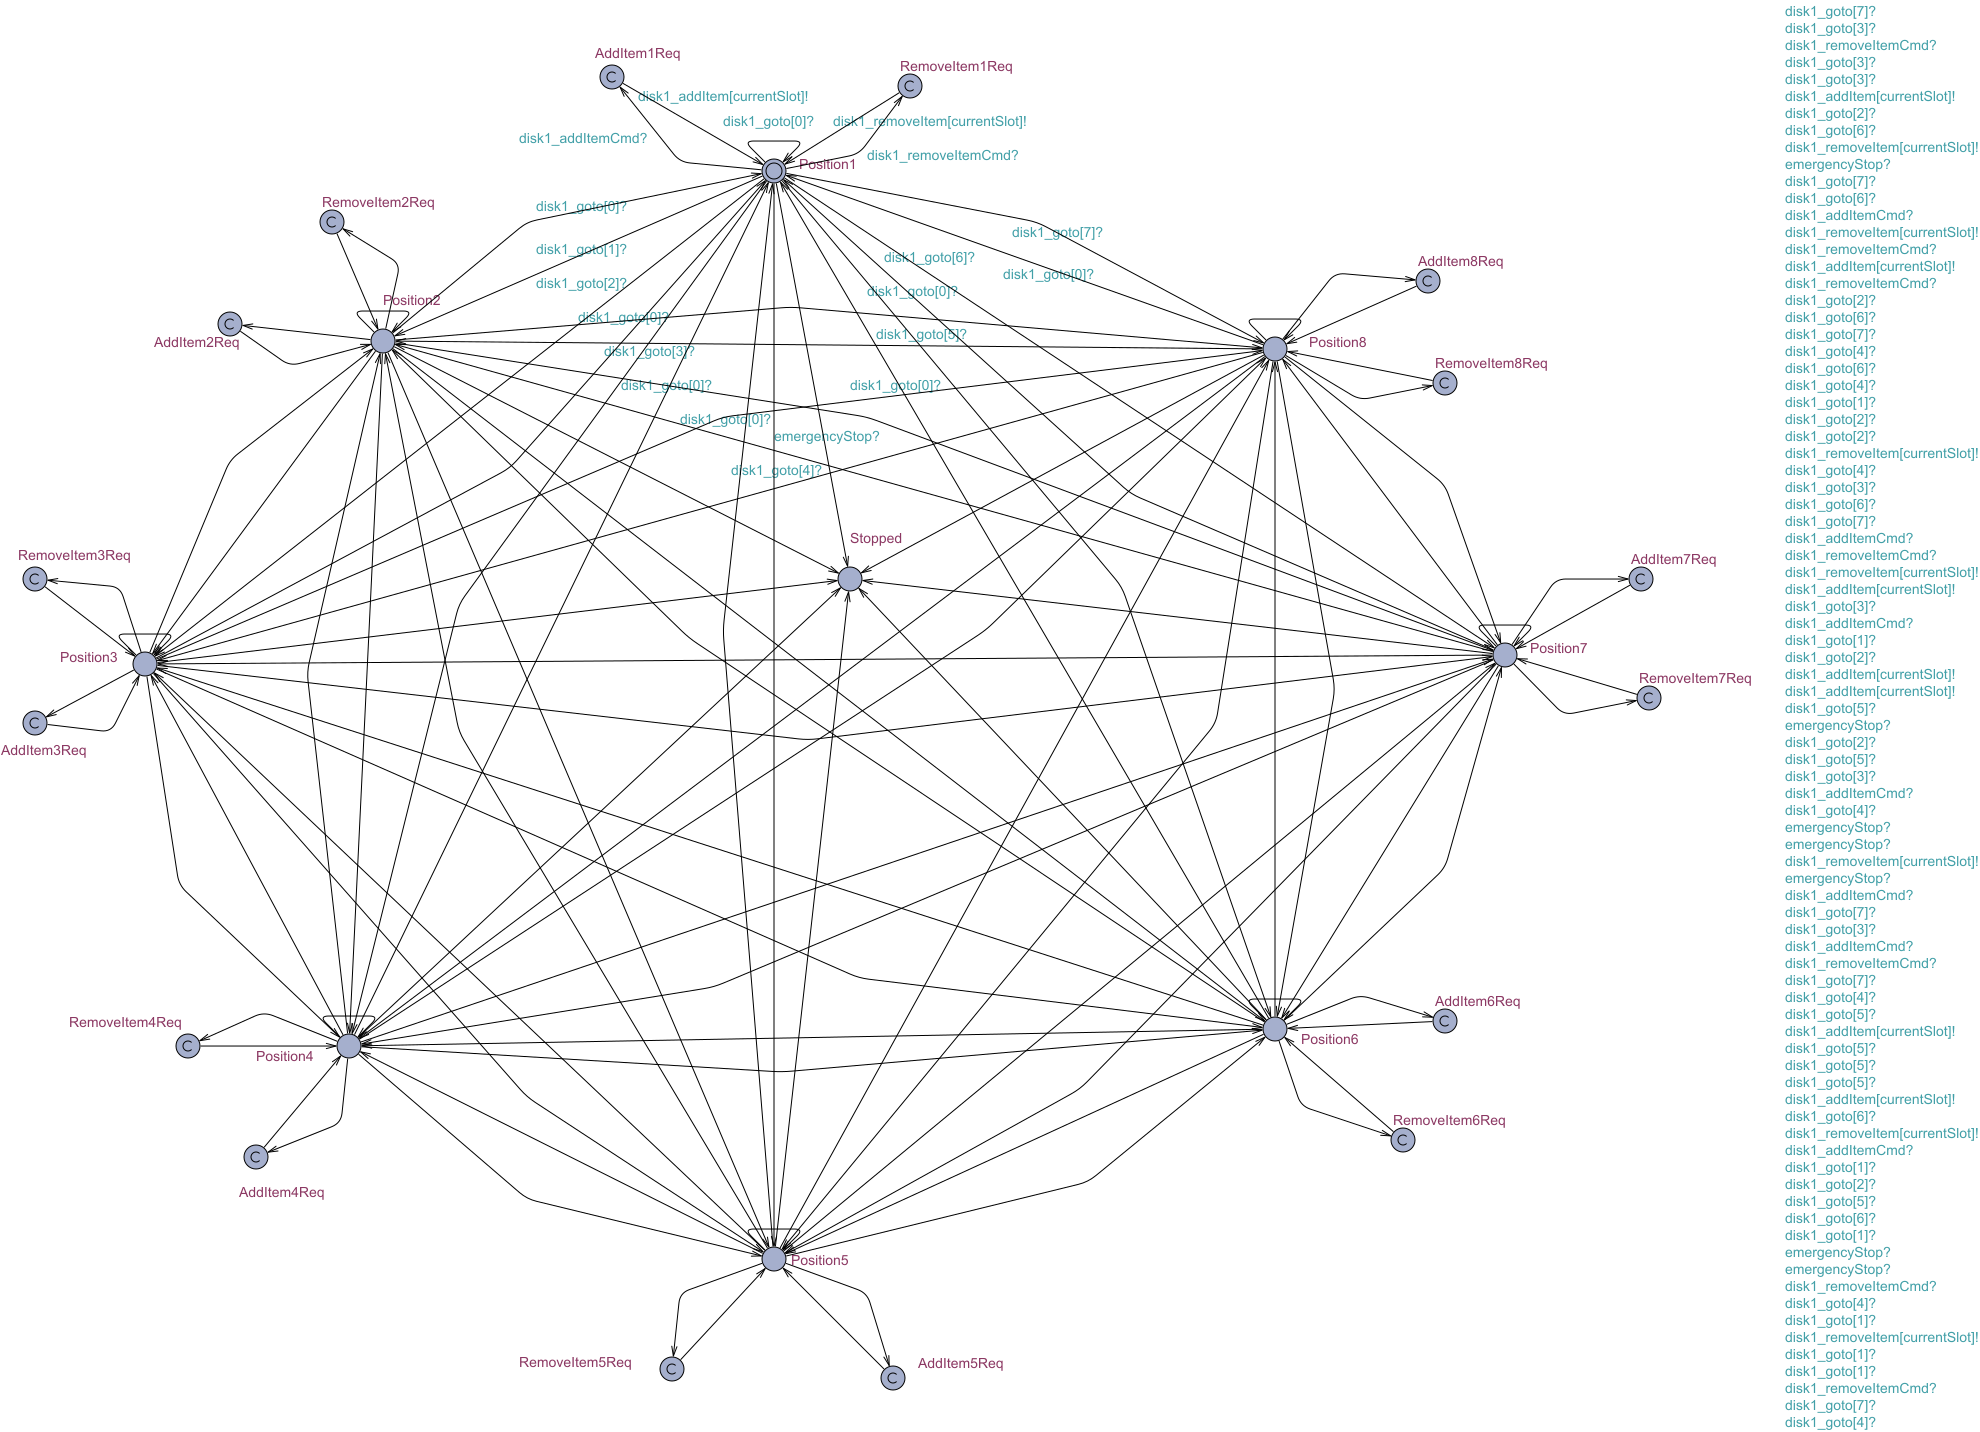
\includegraphics[width=\textwidth]{Image/uppaal-templates/disk1.png}
    \caption{Disk.}
    \label{fig:disk}
\end{figure}

\newpage
\subsection{The Disk Slot template}
\begin{figure}[H]
    \centering
    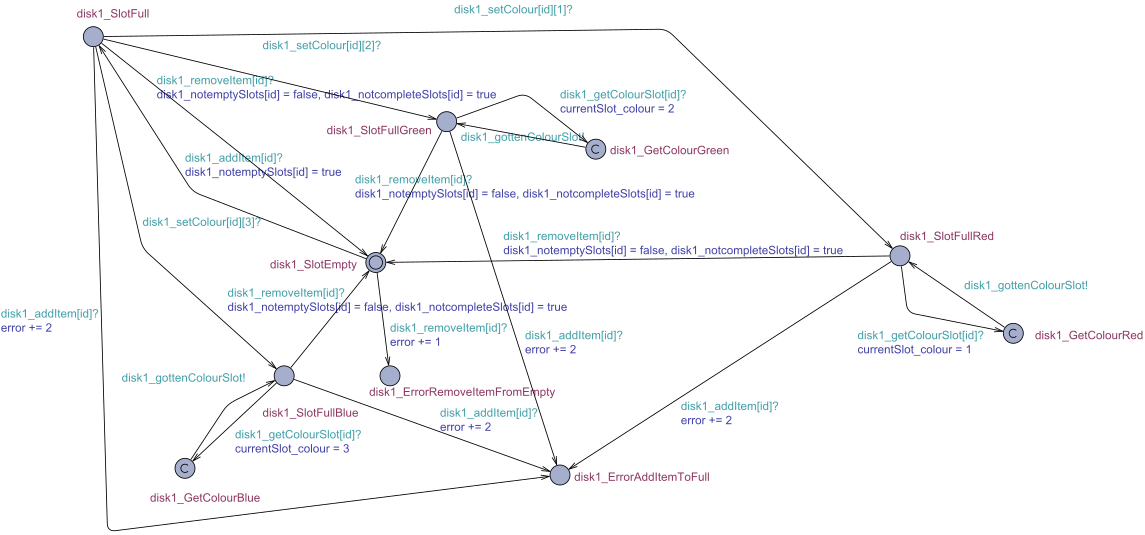
\includegraphics[width=\textwidth]{Image/uppaal-templates/disk1_DiscSlot.png}
    \caption{Disk Slot.}
    \label{fig:disk_slot}
\end{figure}

\newpage
\subsection{The Get Empty Slot template}
\begin{figure}[H]
    \centering
    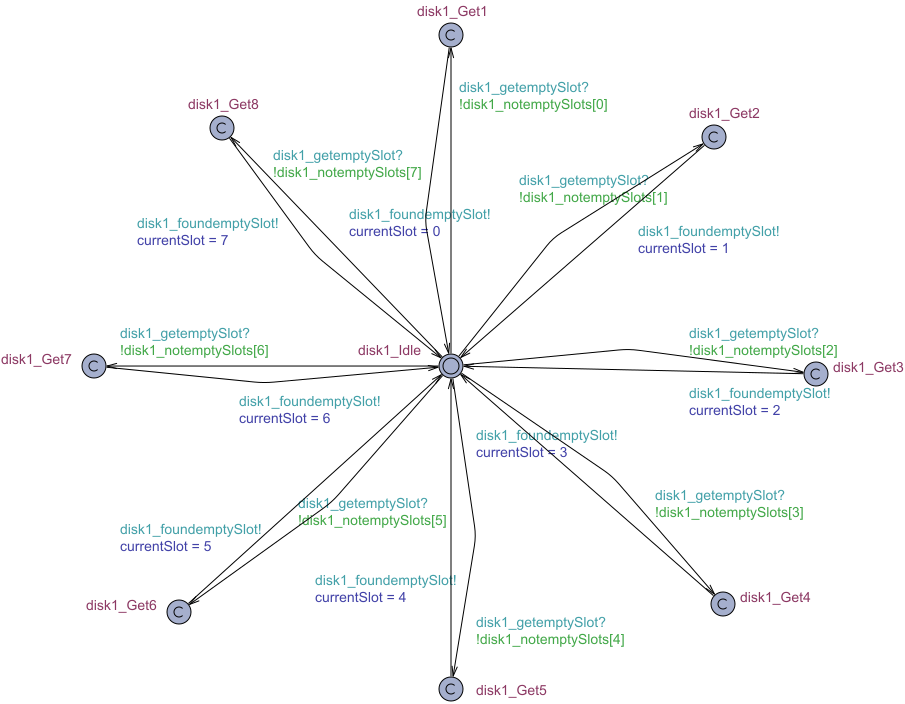
\includegraphics[width=\textwidth]{Image/uppaal-templates/disk1_GetemptySlot.png}
    \caption{Disk - Get Empty Slot.}
    \label{fig:empty_slot}
\end{figure}

\newpage
\subsection{The Get Complete Slot template}
\begin{figure}[H]
    \centering
    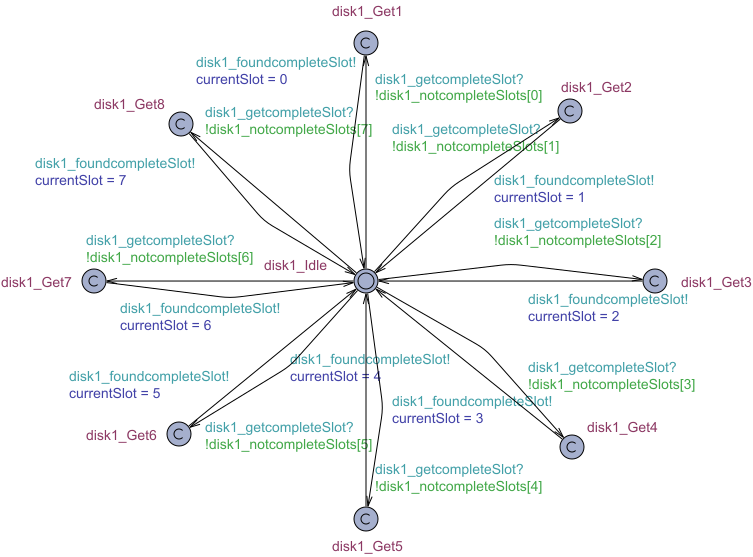
\includegraphics[width=0.8\textwidth]{Image/uppaal-templates/disk1_GetcompleteSlot.png}
    \caption{Disk - Get Complete Slot}
    \label{fig:complete_slot}
\end{figure}

\newpage
\subsection{The Disk Get Free Slot template}
\begin{figure}[H]
    \centering
    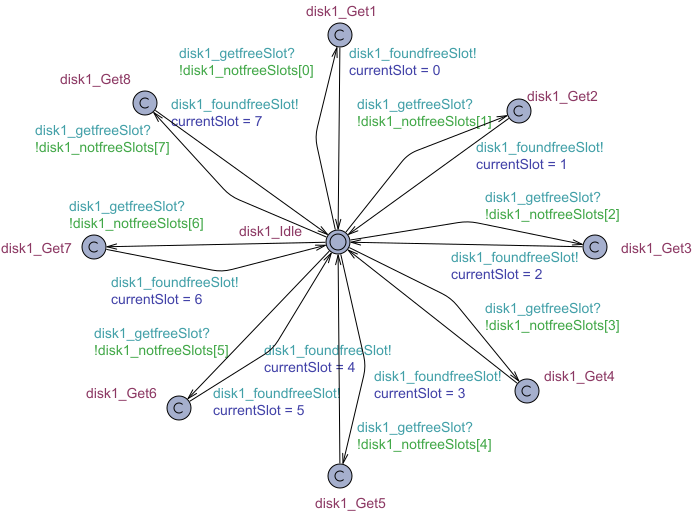
\includegraphics[width=0.8\textwidth]{Image/uppaal-templates/disk1_GetfreeSlot.png}
    \caption{Disk - Get Free Slot}
    \label{fig:free_slot}
\end{figure}

\newpage
\subsection{The Get In Progress Slot template}
\begin{figure}[H]
    \centering
    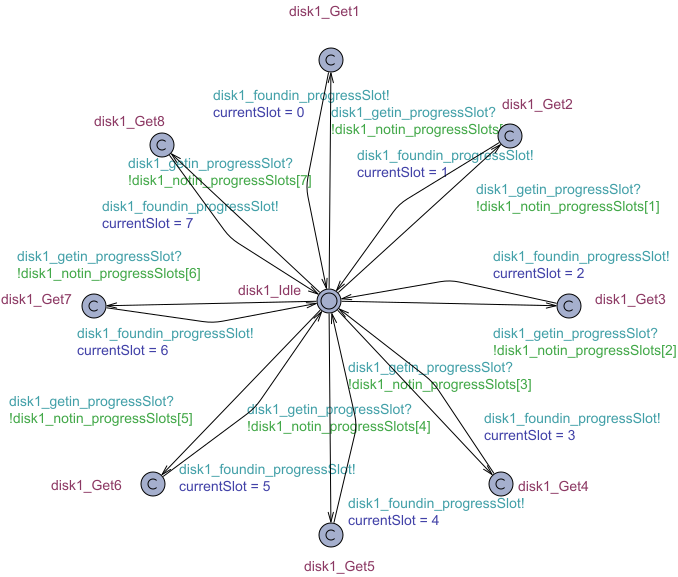
\includegraphics[width=0.8\textwidth]{Image/uppaal-templates/disk1_Getin_progressSlot.png}
    \caption{Disk - Get In Progress Slot}
    \label{fig:in_progress_slot}
\end{figure}

\newpage
\subsection{The Slot Variable - Complete template}
\begin{figure}[H]
    \centering
    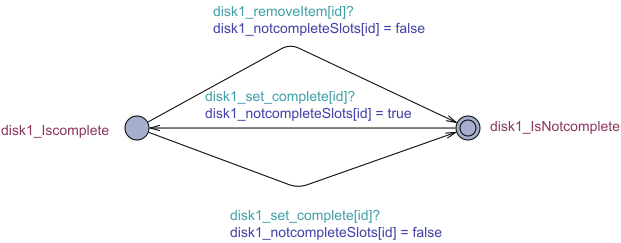
\includegraphics[width=0.7\textwidth]{Image/uppaal-templates/disk1_SlotVariable_complete.png}
    \caption{Disk - Slot Variable Complete}
    \label{fig:slot_variable_complete}
\end{figure}

\subsection{The Slot Variable - Free template}
\begin{figure}[H]
    \centering
    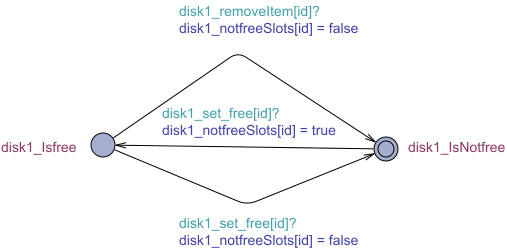
\includegraphics[width=0.7\textwidth]{Image/uppaal-templates/disk1_SlotVariable_free.png}
    \caption{Disk - Slot Variable Free}
    \label{fig:slot_variable_free}
\end{figure}

\subsection{The Slot Variable - In-progress template}
\begin{figure}[H]
    \centering
    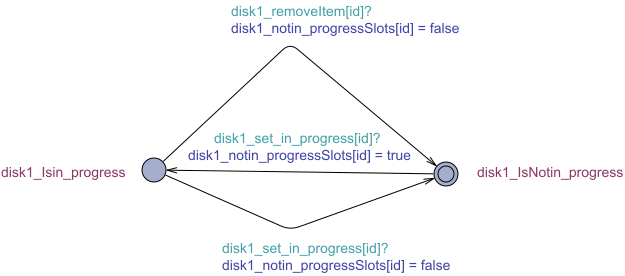
\includegraphics[width=0.7\textwidth]{Image/uppaal-templates/disk1_SlotVariable_in_progress.png}
    \caption{Disk - Slot Variable In Progress}
    \label{fig:slot_variable_in_progress}
\end{figure}

\subsection{The Crane template}
\begin{figure}[H]
    \centering
    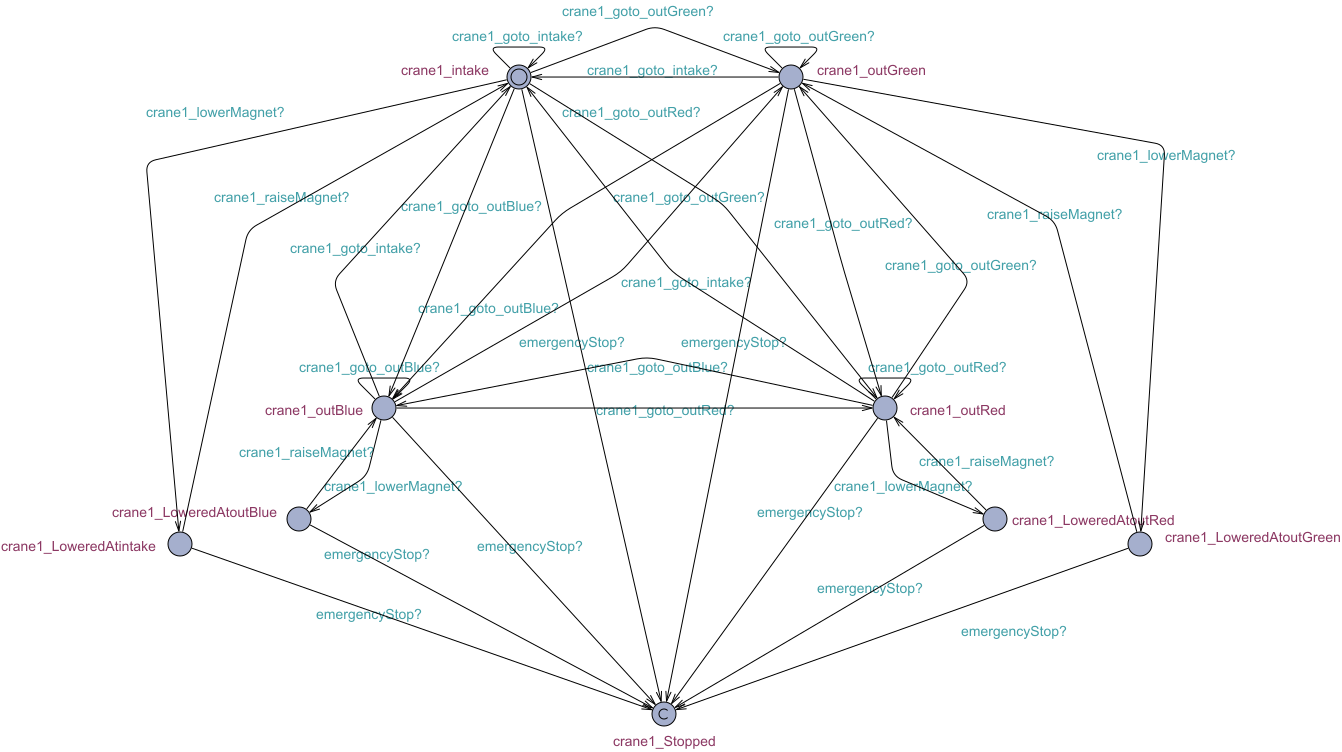
\includegraphics[width=\textwidth]{Image/uppaal-templates/crane1.png}
    \caption{Crane.}
    \label{fig:crane}
\end{figure}

\subsection{The Crane Magnet template}
\begin{figure}[H]
    \centering
    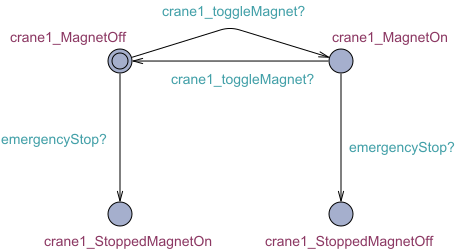
\includegraphics[width=0.5\textwidth]{Image/uppaal-templates/crane1_CraneMagnet.png}
    \caption{Crane Magnet.}
    \label{fig:crane_magnet}
\end{figure}

\subsection{The Camera template}
\begin{figure}[H]
    \centering
    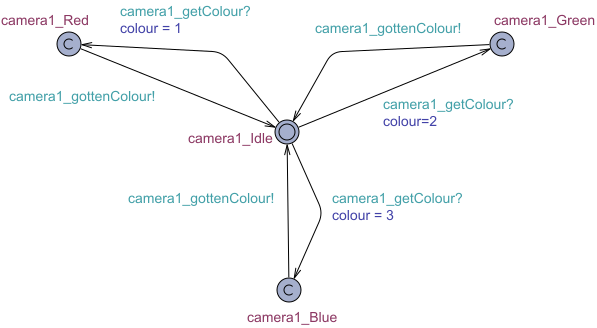
\includegraphics[width=0.75\textwidth]{Image/uppaal-templates/camera1.png}
    \caption{Camera.}
    \label{fig:camera}
\end{figure}

\subsection{The Emergency Button template}
\begin{figure}[H]
    \centering
    
\includegraphics[width=0.5\textwidth]{Image/uppaal-templates/EmergencyButton.png}
    \caption{Emergency Button.}
    \label{fig:emergency_button}
\end{figure}







\end{document}
